\section{METODOLOGI}

% Ubah konten-konten berikut sesuai dengan isi dari metodologi

\subsection{Dataset yang Digunakan}

Data yang digunakan adalah video yang direkam pada beberapa jalan di kota Surabaya lalu
diekstrak menjadi gambar yang akan dianotasikan sesuai dengan format \emph{bounding box}
YOLO.

% Contoh input gambar dengan format *.jpg
\begin{figure} [ht] \centering
  % Nama dari file gambar yang diinputkan
  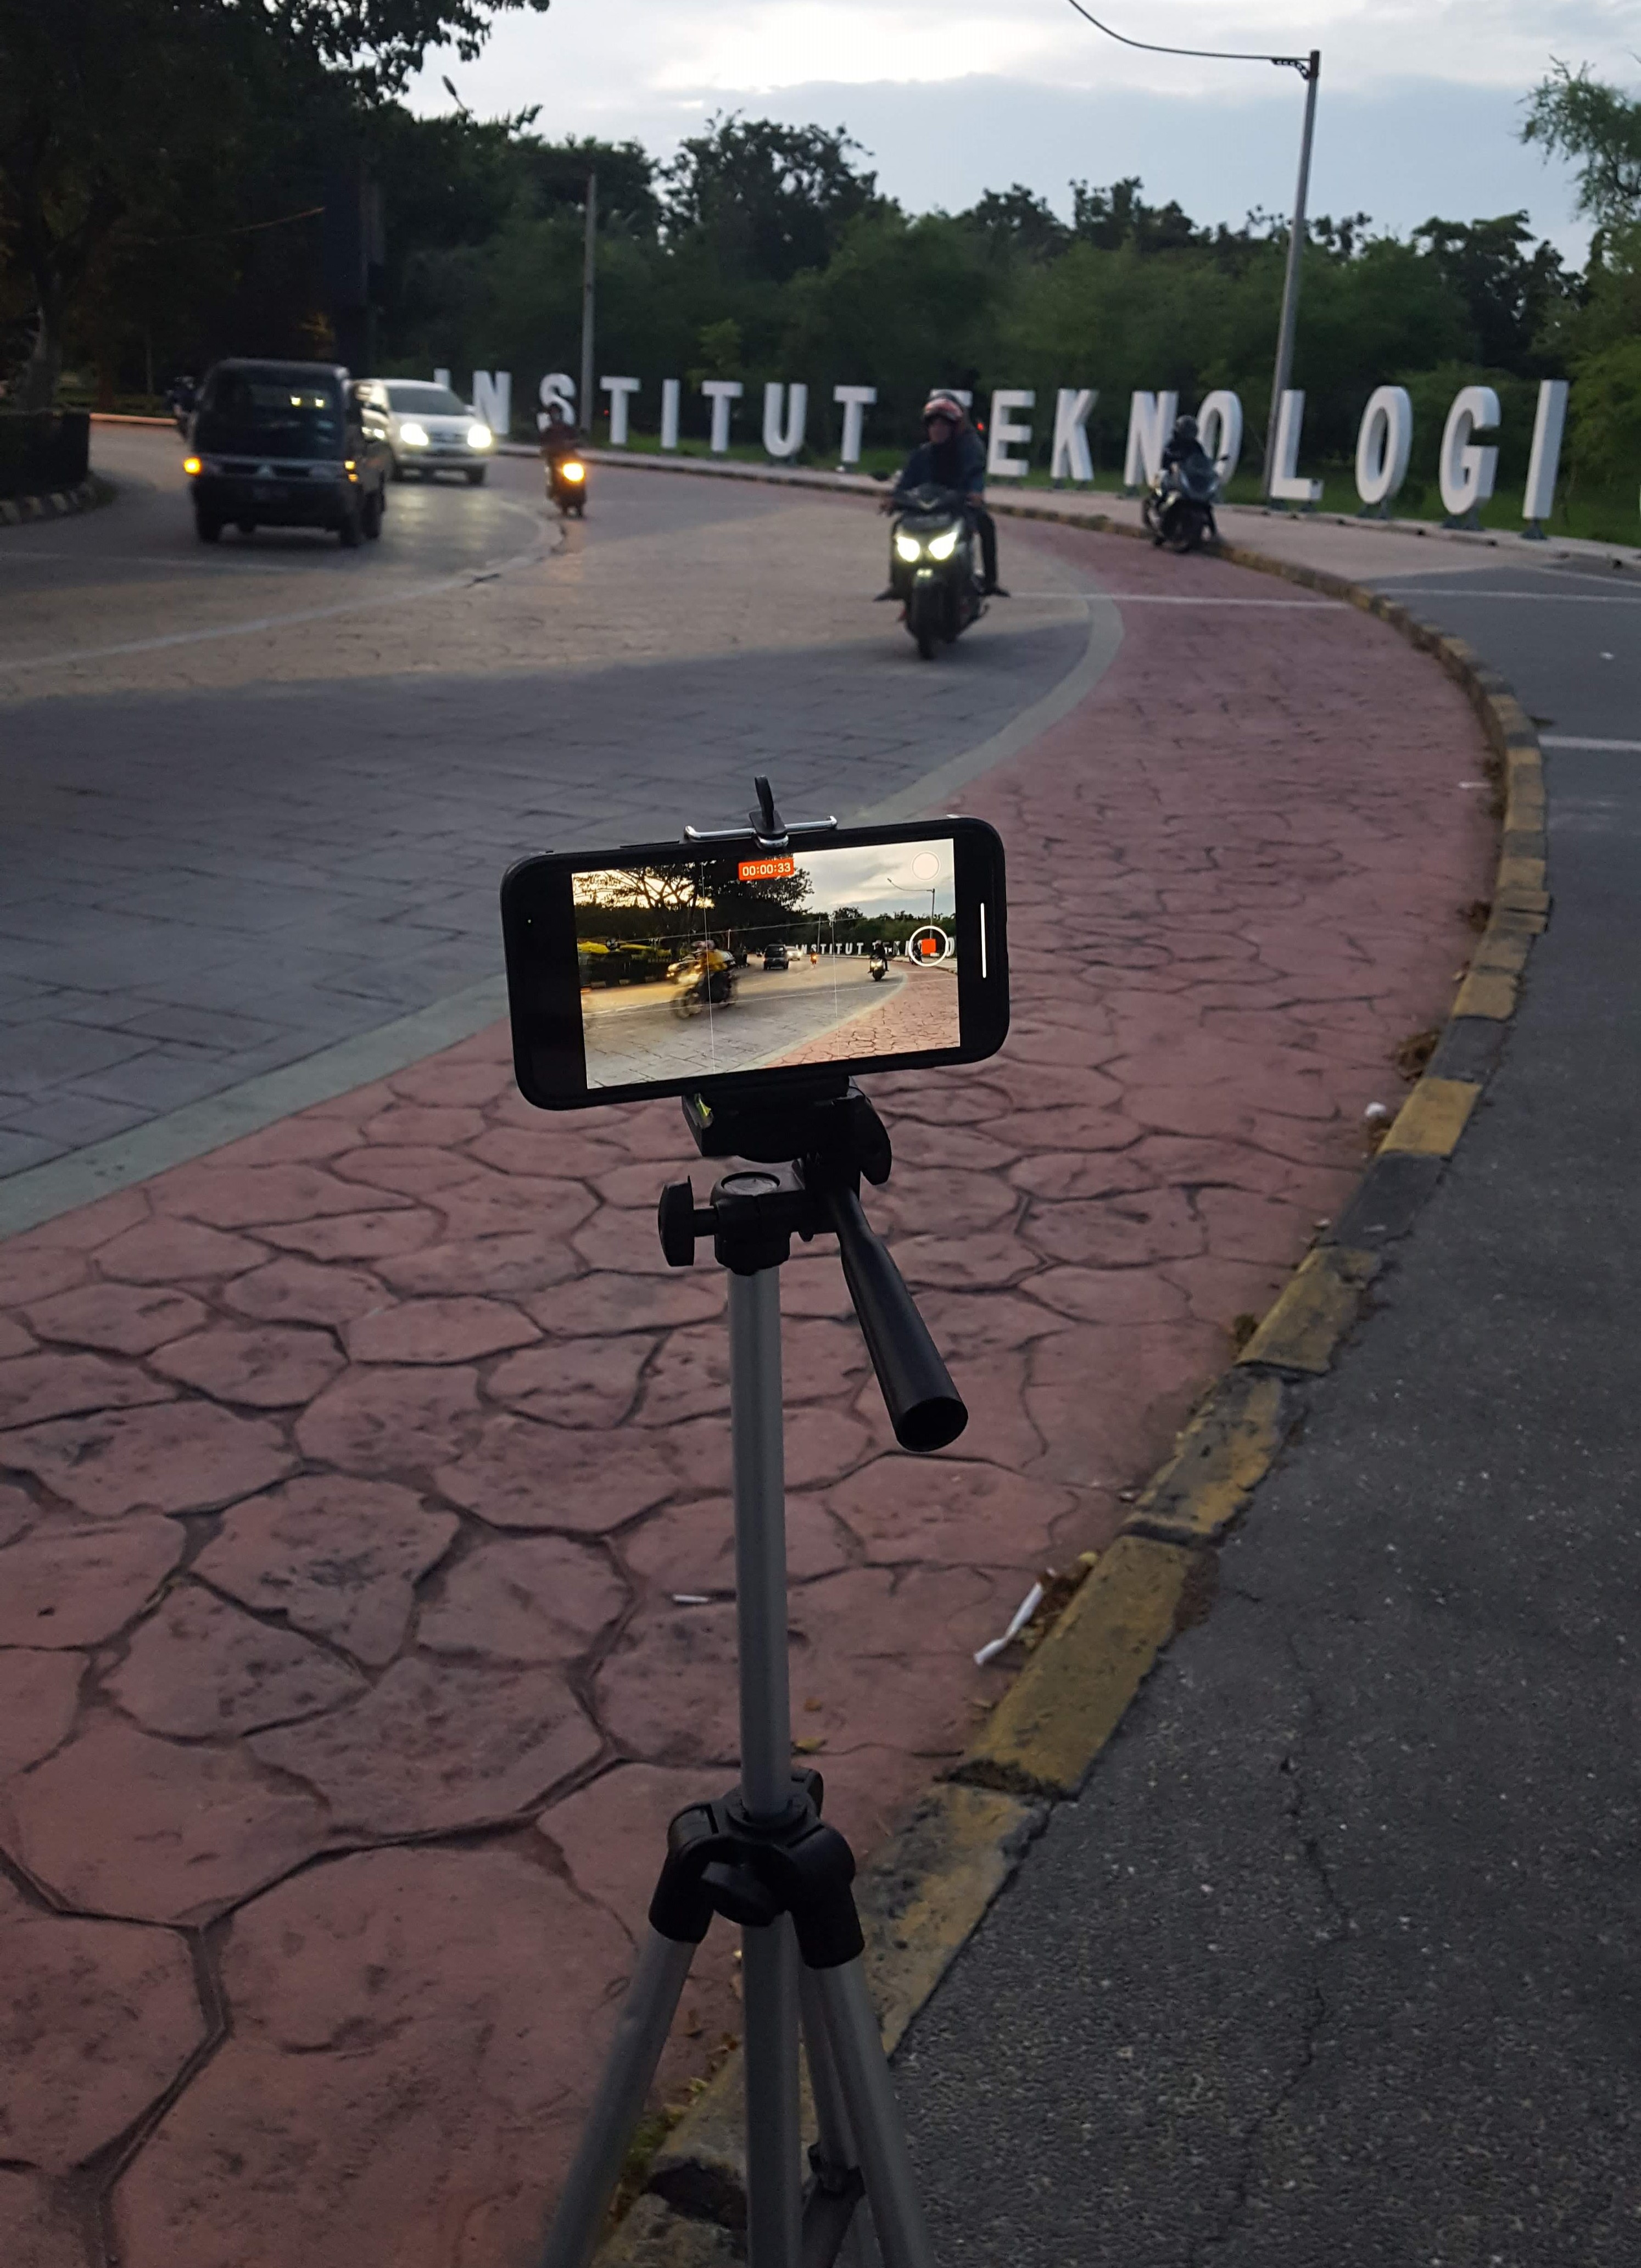
\includegraphics[scale=0.05]{gambar/pengambilan-vide.jpg}
  % Keterangan gambar yang diinputkan
  \caption{Posisi kamera dalam mengambil data video}
  % Label referensi dari gambar yang diinputkan
  \label{fig:pengambilan-video}
\end{figure}

% Contoh penggunaan referensi dari gambar yang diinputkan
Pada tahap pengambilan data video, data video diambil menggunakan kamera pada \emph{smartphone} Apple Iphone XS yang diletakkan pada tepi beberapa jalan raya di kota Surabaya. Kamera \emph{smartphone}
diletakkan pada \emph{tripod} yang memiliki tinggi 1,5 meter. Posisi peletakan kamera pada tripod bisa dilihat pada Gambar \ref{fig:pengambilan-video}.
Setiap video yang diambil menggunakan resolusi 1920 x 1080 \emph{pixels} 30 \emph{frame per second} dengan durasi setiap video 20 menit.


\subsection{Metodologi Penelitian}

Penelitian ini dilaksanakan sesuai sistem berikut dengan implementasinya. Desain
sistem merupakan konsep dari pembuatan dan perancangan infrastuktur yang kemudian diwujudkan
dalam bentuk blok diagram alur yang harus dikerjakan. Pada bagian implementasi merupakan
pelaksanaan teknis untuk setiap blok pada desain sistem. Pada Gambar \ref{fig:diagram-alur} menunjukan bagan umum metodologi
sistem.

\begin{figure} [ht] \centering
  % Nama dari file gambar yang diinputkan
  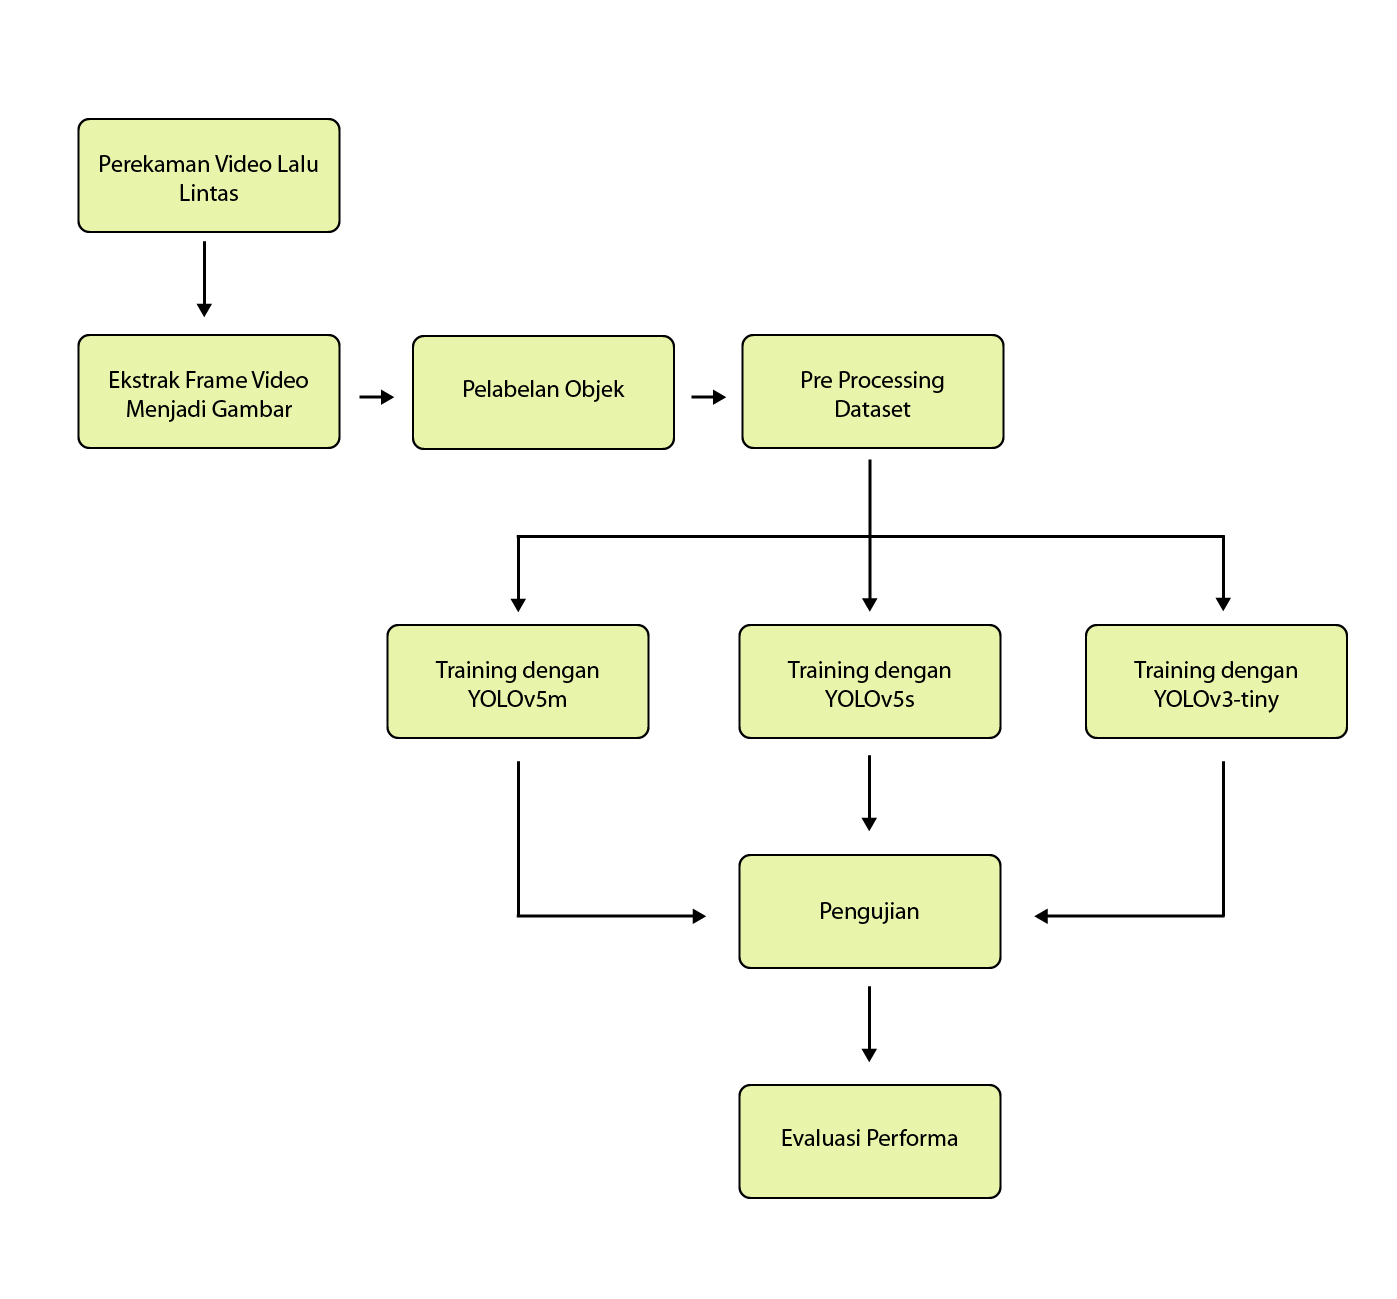
\includegraphics[scale=0.25]{gambar/diagram-pengerjaan-2-100.jpg}
  % Keterangan gambar yang diinputkan
  \caption{Diagram Alur Pengerjaan}
  % Label referensi dari gambar yang diinputkan
  \label{fig:diagram-alur}
\end{figure}

Berdasarkan pada bagan alur metodologi yang dapat dilihat pada Gambar \ref{fig:diagram-alur}, Tahapan pertama yang dilakukan adalah
perekaman video kondisi lalu lintas kota Surabaya. Perekaman video tersebut dilakukan menggunakan perangkat \emph{smartphone} Apple Iphone XS.
Tujuan dari perekaman video tersebut adalah untuk mengumpulkan data yang dibutuhkan untuk proses \emph{training} dan pengujian sistem dari metode yang digunakan.
Dalam sistem ini terdapat tiga objek yang akan dideteksi yaitu adalah pengendara sepeda motor, kepala pengendara sepeda motor menggunakan helm dan kepala pengendara 
sepeda motor tanpa menggunakan helm. Lalu objek tersebut diberikan label atau anotasi yang sesuai kelas yang ditambahkan. Pelabelan data tersebut berupa
\emph{bounding box} yang menunjukkan posisi kelas objek tersebut berdasarkan koordinat resolusinya. Setelah didapatkan data yang lengkap dengan labelnya, lalu data tersebut dapat digunakan
pada proses \emph{training} menggunakan metode deteksi objek berbasis CNN yaitu YOLOv5 dan YOLOv3. \emph{Weight} yang digunakan pada YOLOv5 adalah YOLOv5m dan YOLOv5s, sedangkan
untuk YOLOv3 menggunakan YOLOv3-tiny.
